\documentclass[fontsize=12pt, paper=a4]{report}
\usepackage{amsmath,graphicx}
\setlength{\parindent}{0em}
\setlength{\parskip}{1ex}
\newcommand{\m}[1]{\left[\begin{array}{cc}#1\end{array}\right]}

\title{Linear overlap to volume overlap}

\begin{document}

\maketitle

\chapter{Intro}

The aim of this document is to explain the formulae behind function getOverlapVolume. This function is part of the interaction and returns the effect volume overlap (at the moment assuming spheres). In the next section is the maths behind this formulae and also in the directory is the mathematica notebook to do the calculation (OverlapVolume.nb). 

\chapter{The Math}
%\[\nabla\cdot\sigma = \m{\nabla_n\\\nabla_u}\cdot\m{\sigma_n & \sigma_{nu}\\\sigma_{un} & \sigma_{u}}
%= \m{\nabla_n\sigma_n + \nabla_u\sigma_{nu}\\\nabla_n\sigma_{un} + \nabla_u\sigma_{u}}\]
%\[(\nabla\cdot\sigma)\cdot n = (\nabla\cdot\sigma)\cdot \m{1\\0} = \nabla_n\sigma_n + \nabla_u\sigma_{nu}\]
%If the (shear) stress is uniform (no gradient) in u-direction
%\[(\nabla\cdot\sigma)\cdot n = \nabla_n\sigma_n\]
Given overlap $\delta$ and particle radii $r_1$, $r_2$, we want to the overlap volume $V$.

First we compute the thickness of the spherical caps, $t_1 = r_1-a$ and $t_2 = r_2-b$, in the diagram below.
\begin{center}
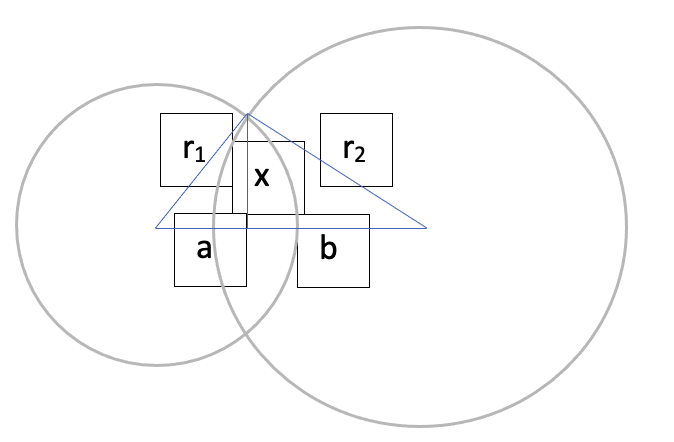
\includegraphics[width=0.5\textwidth]{Schematic}
\end{center}
We know
\[ x^2 = r_1^2 - a^2,\quad x^2 = r_2^2 - b^2,\quad a+b = r_1+r_2-\delta \]
Thus
\[ r_1^2 - a^2 = r_2^2 - (r_1+r_2-\delta-a)^2 \]
Mathematica yields with the following commands:\\
\verb$Simplify[r1 - a /. Solve[r1^2 - a^2 == r2^2 - (r1 + r2 - d - a)^2, a]]$
\begin{equation} 
t_1 = r_1-a = \frac{r_2-\delta/2}{r_1+r_2-\delta}\delta
\end{equation}
\begin{equation} t_2 = r_2-b = \frac{r_1-\delta/2}{r_1+r_2-\delta}\delta
\end{equation}
Thus, the volume of the two spherical caps is
\[V = \pi \left\{\int_0^{t_1} r_1^2-r^2 dr + \int_0^{t_2} r_2^2-r^2 dr\right\}\]
%\[V = \pi \left[[r_1^2r-r^3/3]_0^{t_1} + [r_2^2r-r^3/3 dr]_0^{t_2}\right]\]
\begin{equation}
V = \pi \left\{r_1^2t_1-t_1^3/3 + r_2^2t_2-t_2^3/3\right\}
\end{equation}
It seems, this cannot be simplified further. The full expression in terms of $r_1$, $r_2$, $\delta$ is 
\tiny
\[V = \pi \left\{\frac{-\delta^3 (\delta-2 r_2)^3-12 r_2^2 (-\delta+r_1+r_2)^2 \left(\delta^2-2 \delta (r_1+r_2)+2 r_2 (r_1+r_2)\right)+\left(\delta^2-2 \delta (r_1+r_2)+2 r_2 (r_1+r_2)\right)^3+12 \delta r_1^2 (\delta-2 r_2) (-\delta+r_1+r_2)^2}{24 (\delta-r_1-r_2)^3}\right\}\]


\end{document}